\section{Ignition}
\begin{frame}{Power Balance - Thermonuclear Power}
	For D-T reaction (assuming $n_d=n_t$), the thermonuclear power density is given by
	\begin{equation}
		p_{Tn} = \frac{1}{4}n^2\expval{\sigma v}\varepsilon
		\label{eq:thermonuclear-power-density}
	\end{equation}
	where $n=n_d+n_T$ is the total number of density, and $\expval{\sigma v}$ is drawn in Fig.\ref{fig:sigma-v}, $\varepsilon$ is the energy released per reaction.

	\begin{itemize}
		\item 4/5 of the reaction energy, $\varepsilon$, is carried away by neutrons, the rest is carried by $\alpha$-particles, $\varepsilon_\alpha$.
		\item Neutrons will leave plasma without any interaction.
		\item The $\alpha$-particles will be confined by magnetic field, hence self heating the plasma.
	\end{itemize}
\end{frame}

\begin{frame}{Power Balance - $\alpha$-particle Heating}
	Since the $\alpha$-particles are trapped by the magnetic field, so they will transfer their 3.5MeV energy to the plasma through collisions. Thus, the $\alpha$-particle heating power
	\begin{equation}
		P_\alpha = \int \frac{1}{4}n^2\expval{\sigma v}\varepsilon_\alpha \dd[3]{x} = \frac{1}{4}\overline{n^2\expval{\sigma v}}\varepsilon_\alpha V
		\label{eq:power-alpha}
	\end{equation}
	where the bar means average in the plasma, and $V$ is the volume of the plasma.
\end{frame}

\begin{frame}{Power Balance - Energy Loss}
	Since each plasma particle has energy $3T/2$ ($T/2$ in each degree of freedom), and there are equal number of electrons and ions, so the total energy of the plasma is
	\begin{equation}
		W = \int 3nT\dd[3]{x} = 3\overline{nT}V
	\end{equation}
	where $V$ is the volume of the plasma.

	If the energy confinement time is $\tau_E$, then the energy loss power is
	\begin{equation}
		P_L = W/\tau_E
		\label{eq:power-loss}
	\end{equation}

	\begin{itemize}
		\item To experimentally determine $\tau_E$, we can maintain a steady state plasma by external heating. In this case the power of energy loss can be estimated by the power of heating, $P_L = P_H$, so
		      \[ \tau_E = W/P_H \]
	\end{itemize}
\end{frame}

\begin{frame}{Ignition - Condition}
	The requirement for the plasma burn to be self-sustaining is
	\begin{equation}
		P_\alpha > P_L
	\end{equation}
	Take constant density and temperature for simplicity, we have
	\begin{equation}
		n\tau_E > \frac{12 T}{\expval{\sigma v} \varepsilon_\alpha}
	\end{equation}
	The right-hand-side of the inequality is drawn in Fig.\ref{fig:ignition-condition}.

	Since $\tau_E$ itself is also a function of temperature, so there is a more convenient form,
	\begin{equation}
		nT\tau_E > 3\times10^{21} \text{keV\cdot s}
	\end{equation}
\end{frame}

\begin{frame}{Ignition - Condition}
	\begin{figure}
		\centering
		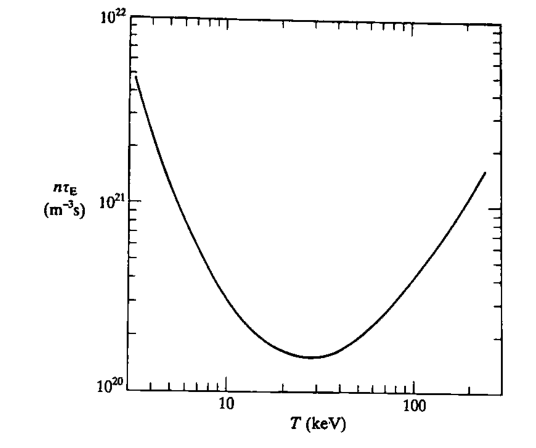
\includegraphics[width=0.6\textwidth]{figures/ignition-condition.png}
		\caption{Adapted from \cite{wesson_campbell_tokamaks_2011}. The value of $n\tau_E$ required to obtain ignition, as a function of temperature.}
		\label{fig:ignition-condition}
	\end{figure}
\end{frame}

\begin{frame}{Ignition - Approach}
	\begin{itemize}
		\item L-mode: Low confinement mode. Poor confinement in this regime.
		\item H-mode: High confinement mode. $\tau_E$ of plasma is long in this regime.
		\item With high enough applied power, plasma transition from L to H-mode.
		\item Once the mode transition happens, the plasma burn is self-sustaining.
	\end{itemize}
	\begin{figure}
		\centering
		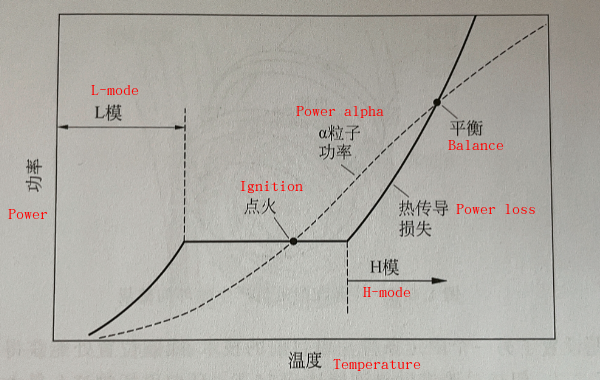
\includegraphics[width=0.6\textwidth]{figures/ignition-approach.png}
		\caption{Adapted from \cite{wesson_campbell_tokamaks_2011}. $P_L$ and $P_\alpha$ as function of temperature.}
	\end{figure}
\end{frame}